\documentclass[a4paper,10pt]{article}
\usepackage[utf8]{inputenc}

\usepackage[margin=2cm,headheight=26pt,includeheadfoot]{geometry}

\usepackage[german]{babel}
\usepackage[german=quotes]{csquotes}

\usepackage{nameref}
\usepackage{microtype}
\usepackage{float}
\usepackage{siunitx}
\sisetup{
    locale = DE,
    binary-units,
    detect-all, 
    per-mode = symbol %enables m/s instead of ms^-1
}
\AtBeginDocument{\DeclareSIUnit{\kWh}{kWh}}

\usepackage{caption} %for \caption*
\usepackage{hhline}
\usepackage{tabularx}
\usepackage{array}
\usepackage{calc}
\usepackage{multicol}
\usepackage{multirow}
\usepackage{parskip}
\usepackage{booktabs}

\usepackage{fancyhdr}
\pagestyle{fancy}
\setlength{\headheight}{48pt}
\renewcommand{\headrulewidth}{0pt}

\usepackage{xcolor,colortbl}
\usepackage{makecell}

\usepackage[symbol*]{footmisc}
\renewcommand{\thefootnote}{\fnsymbol{footnote}}
\renewcommand{\thempfootnote}{\fnsymbol{mpfootnote}}

\usepackage{color} 
\usepackage{enumitem}

\usepackage{pdfpages}

% Word-Stealth-Modus, kann aber kein Omega
%\usepackage[scaled]{helvet}

\usepackage[inline,nomargin]{fixme}
\fxsetup{
    author=,
    layout=inline,
    theme=color
}

\definecolor{fxnote}{rgb}{0.8000,0.0000,0.0000}
\colorlet{fxnotebg}{yellow}

\definecolor{boxgray}{rgb}{0.33,0.33,0.33}
\definecolor{boxred}{rgb}{0.8,0,0}
\usepackage{tcolorbox}
\title{}
\author{}

\renewcommand{\familydefault}{\sfdefault}

\newcommand{\hint}[1]{\begin{tcolorbox}[colback=boxgray,colframe=black,coltext=
white,title=Hinweis]#1\end{tcolorbox}}

\newcommand{\warn}[1]{\begin{tcolorbox}[colback=boxred,colframe=red,coltext=
white,title=Warnung]#1\end{tcolorbox}}

\newcommand{\gfx}[1]{\includegraphics[width=\linewidth]{#1}}

\newcommand*{\fullref}[1]{\hyperref[{#1}]{\ref*{#1}~\nameref*{#1}}}

\fancyhf{}
\fancyhead{\colorbox{boxgray}{
    \makebox[\dimexpr\linewidth-2\fboxsep][l]{
        
\includegraphics[height=1cm]{./img/logo}\hfill\color{white}\Huge\raisebox{.5ex}{\thepage}
        }
    }
}

\usepackage{hyperref}
\usepackage{qrcode}

\appto\UrlNoBreaks{\do\.\do\:\do\/\do\_}

\usepackage{hyphenat}

\begin{document}
\pagestyle{empty}
\begin{titlepage}
	\vspace*{-3.08cm}
	\colorbox{boxgray}{\makebox[\dimexpr\linewidth-2\fboxsep][c]{
\includegraphics[width=0.6\textwidth]{./img/logo}}}
	\vfill
	\begin{center}
		\Huge
		WARP Ladesäule Betriebsanleitung\\\vspace{1cm}
		\large
		Version 1.0.0\\\vspace{0.25cm}
		\today
	\end{center}
	\vfill
	\begin{center}
		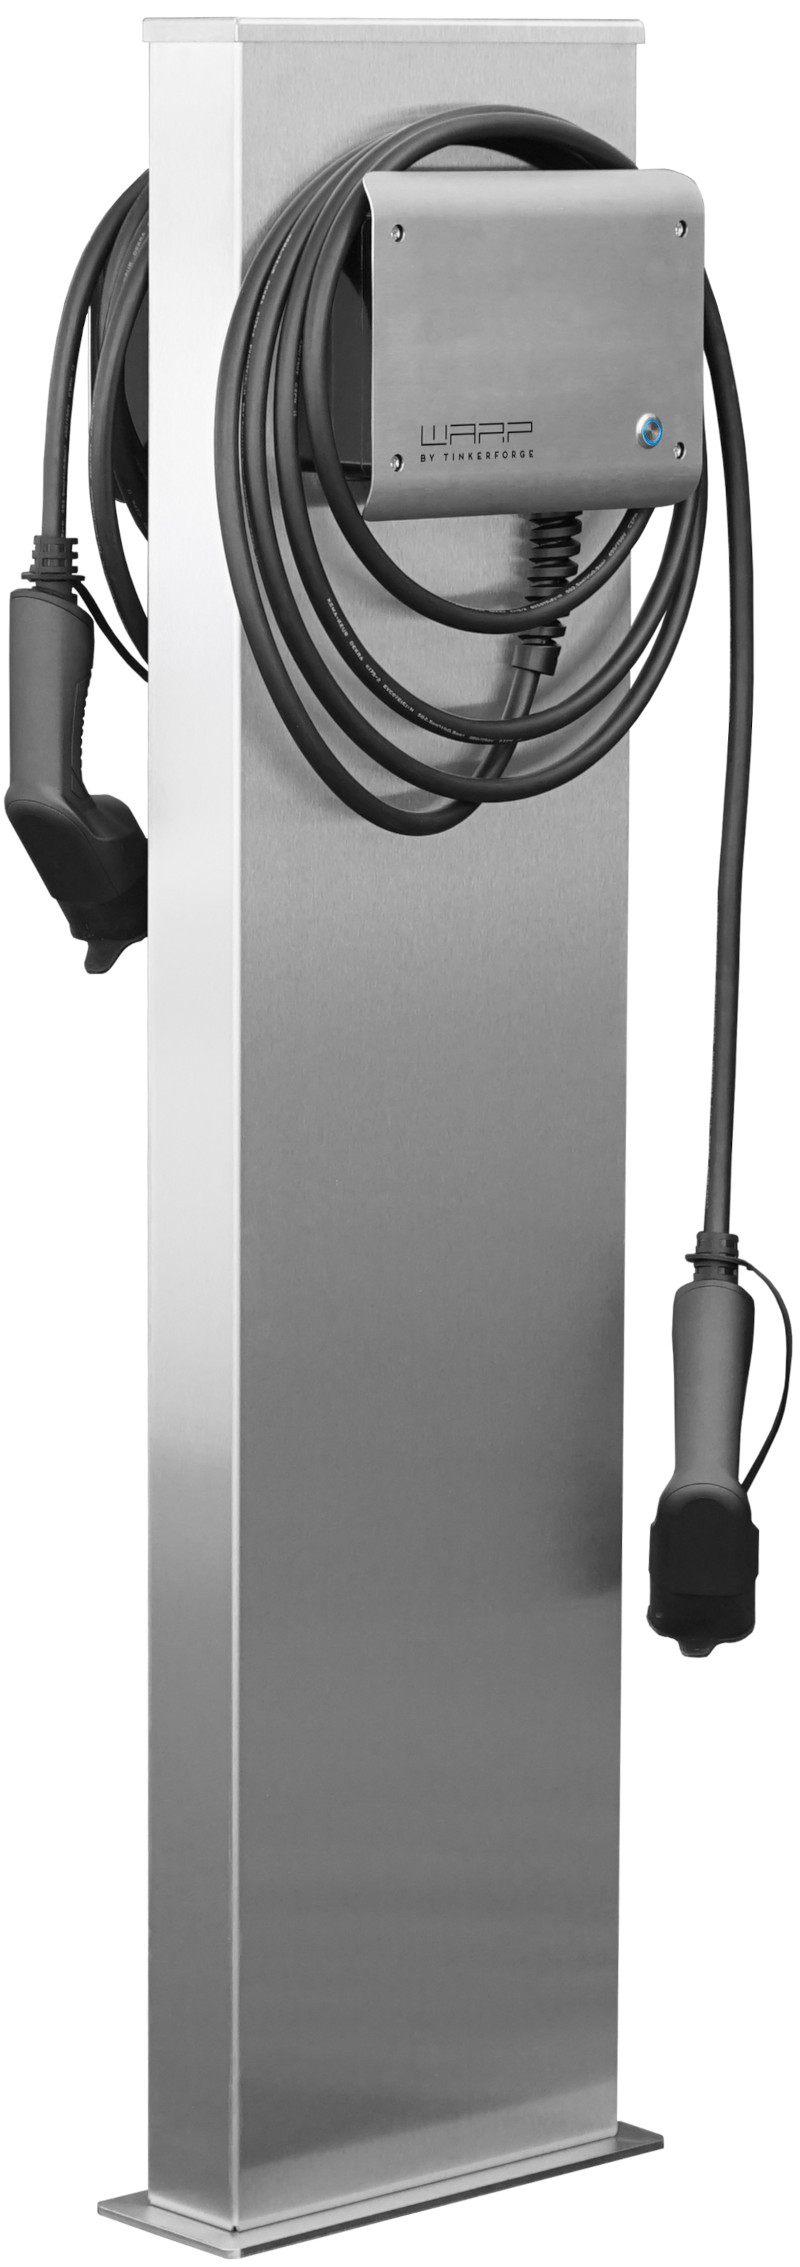
\includegraphics[width=0.3\linewidth]{./img/warp-charger-stand-side}
	\end{center}
\end{titlepage}
\newpage
\null
\newpage
\pagestyle{fancy}
\begin{multicols*}{2}
	\tableofcontents \section{Einführung}
	\subsection{Vorwort} Vielen Dank, dass du
	dich für eine WARP Ladesäule von Tinkerforge entschieden hast!

	\enquote{WARP} steht
	für \textbf{W}all \textbf{A}ttached
	\textbf{R}echarge \textbf{P}oint. Mit der WARP Ladesäule
	erhältst du eine hochqualitative und langlebige Ladesäule, mit der du dein
	Elektrofahrzeug laden kannst. Die Ladesäule ist so aufgebaut, dass
	einzelne Komponenten einfach ausgetauscht werden können. Sowohl Hardware als
	auch Software sind Open Source. Die nachfolgende Betriebsanleitung gibt dir
	alle notwendigen Informationen zu Sicherheit, Montage, Installation, Betrieb
	und Wartung der Ladesäule.

	\subsection{Beschreibung}
	
	Die WARP Ladesäule kann mit einem oder zwei WARP Charger Wallboxen 
	ausgestattet werden (modellabhängig). Die Ladesäule besteht aus
	\SI{1.5}{\milli\meter} starkem V4A Edelstahl und ist mit IP54 für den
	Außenbereich geeignet. Über die geteilte Rückwand kannst du einfach
	die Zuleitungen erreichen und die Ladesäule anschließen. Über eine
	mitgelieferte Montagehilfe, die die Befestigungsschrauben bereits im
	richtigen Abstand positioniert, kann einfach das Betonfundament vorbereitet
	werden. Die Säule kann dann nach Fertigstellung des Fundaments und ggf.
	Erdarbeiten schnell montiert und angeschlossen werden.

	\section{Sicherheitshinweise}
	\subsection{Allgemein}
	Die WARP Ladesäule ist so konstruiert, dass ein sicherer Betrieb gewährleistet ist,
	wenn sie korrekt installiert wurde, in einem einwandfreien technischen Zustand
	ist und diese Betriebsanleitung befolgt wird. \hint{Die Ladesäule darf nur von einer ausgewiesenen Elektrofachkraft installiert
		werden.}

	\subsection{Bestimmungsgemäße Verwendung}
	Der Standfuß dient zur Aufnahme von TinkerForge WARP Ladestationen auf einer freien Fläche, wo eine 
	Wandmontage nicht möglich ist. Es dürfen nur TinkerForge WARP Charger
	Wallboxen an der Ladesäule montiert werden. Den Installations- und
	Verwendungshinweise zu den verwendeten WARP Chargern ist Folge zu leisten.
	Diese sind in der Betriebsanleitung der WARP Charger zu finden.

	Die Ladesäule ist in zwei Produktvarianten erhältlich:
	\begin{itemize}
		\item Aufnahme einer TinkerForge WARP Ladestation.
		\item Aufnahme von zwei TinkerForge WARP Ladestationen.
	\end{itemize}
	
	Bei Variante 2 ist es nicht zulässig, nur eine Ladestation zu montieren und den anderen Platz leer zu lassen.

	\subsection{Allgemeine Sicherheitshinweise}

	Die WARP Ladesäule wurde gemäß den relevanten Sicherheits- und Umweltvorschriften und -bestimmungen 
	entwickelt, hergestellt, geprüft und dokumentiert. Das Gerät nur in technisch einwandfreiem Zustand verwenden.

	Störungen, die die Sicherheit von Personen oder des Geräts beeinträchtigen, 
	sofort von einer autorisierten Elektrofachkraft nach den national geltenden Regeln beheben zu lassen.

	\warn{Nichtbeachtung der Sicherheitshinweise kann zu Lebensgefahr,
	Verletzungen und Schäden am Gerät führen! Der Hersteller lehnt jede Haftung
	für daraus resultierende Ansprüche ab!
	\\
	\\
	\textbf{Elektrische Gefahr!}\\
	Die Montage, erste Inbetriebnahme und Wartung der Ladestation darf nur von einer einschlägig ausgebildeten, qualifizierten und befugten Elektrofachkraft durchgeführt werden, die dabei für die Beachtung der bestehenden Normen und Installationsvorschriften verantwortlich ist. Halten Sie die angeführten Vorgaben für die Standortauswahl und die baulichen Voraussetzungen ein! Abweichungen zu den Standortvorgaben können zu Tod, schweren Körperverletzungen oder Sachschäden führen, wenn die entsprechenden Vorsichtsmaßnahmen nicht getroffen werden!
	}

	\section{Montage und Installation}
	\subsection{Montage}
	\subsubsection{Lieferumfang}
	Im Lieferumfang der Ladesäule befinden sich:
	\begin{itemize}
		\item Edelstahl Standfuß
		\item gewählte WARP2 Charger Wallboxen inkl. Zubehör
		\item Montagehilfe bestehend aus
			\begin{itemize}
				\item 1x Montagehilfe-3D gedruckte Schablone
				\item 4x M8 Schrauben
				\item 4x Scheiben
				\item 8x M8 Muttern
			\end{itemize}
		\item Diese Betriebsanleitung, Betriebsanleitung der Wallboxen,
		Testprotokoll
	\end{itemize}

	\subsubsection{Montageort}

	Folgende Anforderungen müssen zur Montage der WARP Ladesäule erfüllt sein:
	\begin{itemize}
		\item Der Einbauort muss alle Anforderungen erfüllen, die in der
		TinkerForge WARP Bedienungsanleitung aufgeführt sind.
		\item Bei Installation des Standfußes an einer Straße oder einem
		öffentlichen Parkplatz, offen oder überdacht, muss ein entsprechender 
		Anfahr-/Rammschutz angebaut werden.
		\item Sollen mehrere Standfüße nebeneinander installiert werden, muss
		der Abstand zwischen den einzelnen Standfüßen mind. \SI{200}{\milli\meter} betragen.
		\item Die Oberfläche muss vollständig plan sein.
	\end{itemize}

    \hint{Den Standfuß nicht auf Asphalt installieren. Auf Asphalt ist die
	Standsicherheit des Standfuß nicht gewährleistet.}


	\subsubsection{Herstellung des Fundaments}
    Zur sicheren Installation des Standfußes wird ein Betonsockel empfohlen.
	Auslegung, Konstruktion und Ausführung des Sockels sind Aufgabe des 
	Herstellers des Betonsockels und ist ggf. den örtlichen Gegebenheiten
	anzupassen.
	\par
	Im Anhang auf Seite~\ref{appendix_base} findet sich eine detaillierte
	Abbildung zur Herstellung des Fundaments. Die Größe des Betonfundaments ist als
	Mindestgröße anzusehen um einen sicheren Stand zu gewährleisten.
	\par
	Die Montagehilfe muss wie angegeben mit den mitgelieferten Schrauben,
	Scheiben und Muttern aufgebaut werden. Die angegebenen Maße sind
	einzuhalten. Anschließend kann die so aufgebaute Montagehilfe im 
	Betonfundament positioniert werden.
	\par
	Es darf sich kein Wasser am Sockel ansammeln, dieses muss abfließen können. Die 
	Stromversorgungskabel, ein Erdungskabel und ggf. vorhandene Netzwerkkabel müssen in der Mitte 
	des Betonsockels austreten und eine überstehende Länge von mindestens
	\SI{1500}{\milli\meter} haben. Der Sockelhersteller muss
	für einen ausreichenden Schutz der Kabel sorgen. Schutzhüllen müssen mind.
	\SI{250}{\milli\meter} aus dem Beton herausreichen. Ein Erdungsanschluss ist
	zwingend erforderlich.

	\subsubsection{Montage des Standfußes}
	Nachdem der Betonsockel gegossen wurde und ausgehärtet ist, kann
	der Standfuß montiert werden. Bei dem Standfuß sollten zuvor die Rückseiten 
	entfernt werden. Die bei der Montagehilfe
	eingesetzten oberen M8 Muttern (4 Stück) und die Scheiben müssen nun wieder losgeschraubt werden, 
	damit die Gewinde offen liegen. Anschließend kann der Standfuß mittig über den
	Kabeln, welche aus dem Fundament ragen, positioniert werden. Die
	einbetonierte Montagehilfe sorgt für die korrekte Position der
	Befestigungsschrauben. Nach dem Auftstellen des Standfußes auf die Schrauben kann dieser
	mittels der zuvor entfernten Scheiben und Muttern auf das Fundament
	geschraubt werden.

	Die Abbildung auf Seite~\ref{appendix_erection} findet sich eine
	detaillierte Abbildung zu diesem Arbeitsschritt.

	\subsection{Elektrischer Anschluss}
	Der elektrische Anschluss der Wallboxen erfolgt für jede Wallbox separat.
	Es sind die Hinweise der Elektroinstallation der WARP2 Charger aus deren
	Betriebsanleitung zu beachten.

	\subsubsection{Anforderungen an die Elektroinstallation}
	Es sind die Anforderungen an die Elektroinstallation der gewählten WARP2
	Charger Wallboxen zu beachten. Diese sind der mitgelieferten
	Betriebsanleitung zu entnehmen.

	\subsubsection{Elektrische Installation}
	Werksseitig ist jede Wallbox bereits mit einer Anschlussleitung
	ausgestattet und wird über das mitgelieferte Verteilergehäuse
	angeschlossen.

	\begin{center}
		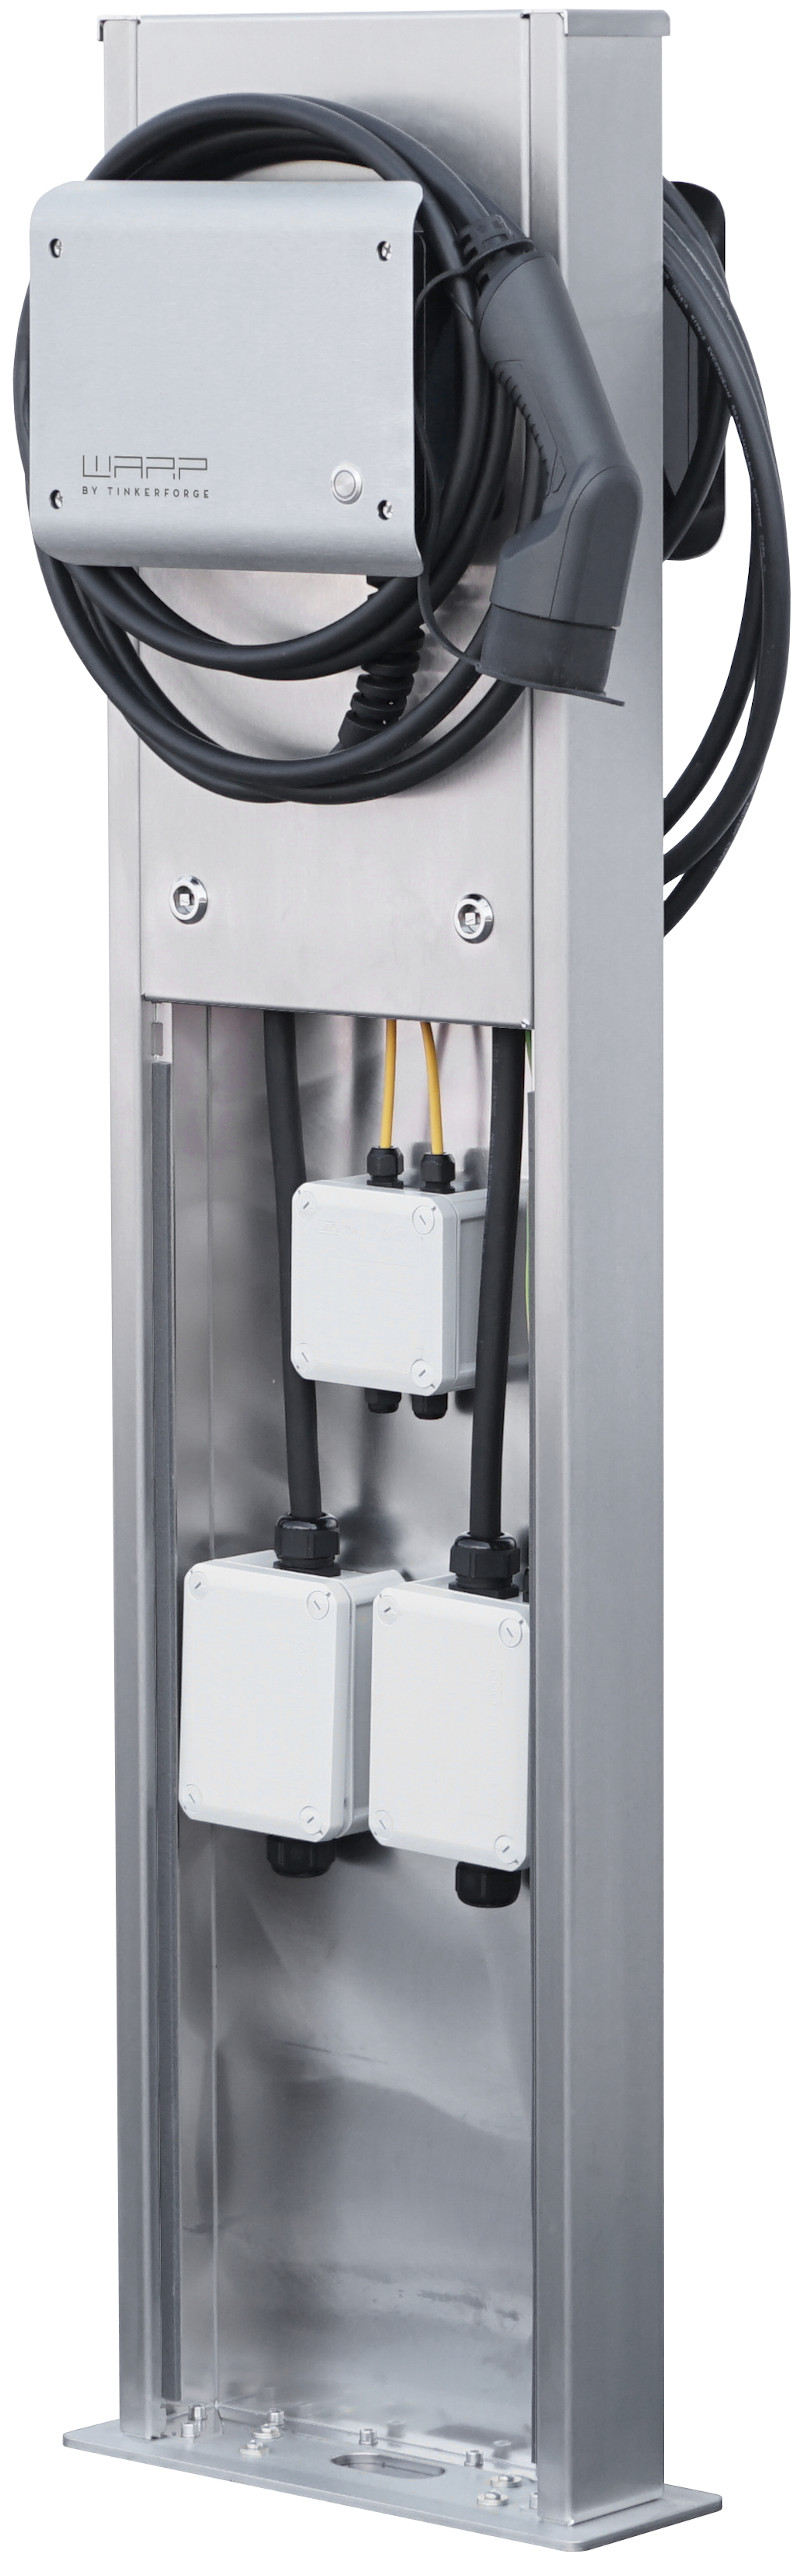
\includegraphics[width=0.3\linewidth]{./img/warp-charger-stand-back-opened}
	\end{center}

	In dem Verteilergehäuse befinden sich Klemmen vom Typ SRK 10
	oder vergleichbar. Es können ein- und mehrdrähtiger Leiter mit bis zu
	\SI{16}{\square\milli\meter} und Leiter mit Aderendhülse mit einem
	Querschnitt von bis zu \SI{10}{\square\milli\meter} angeschlossen werden.
	Die Abisolierlänge beträgt \SI{10}{\milli\meter}.
	

	\begin{center}
		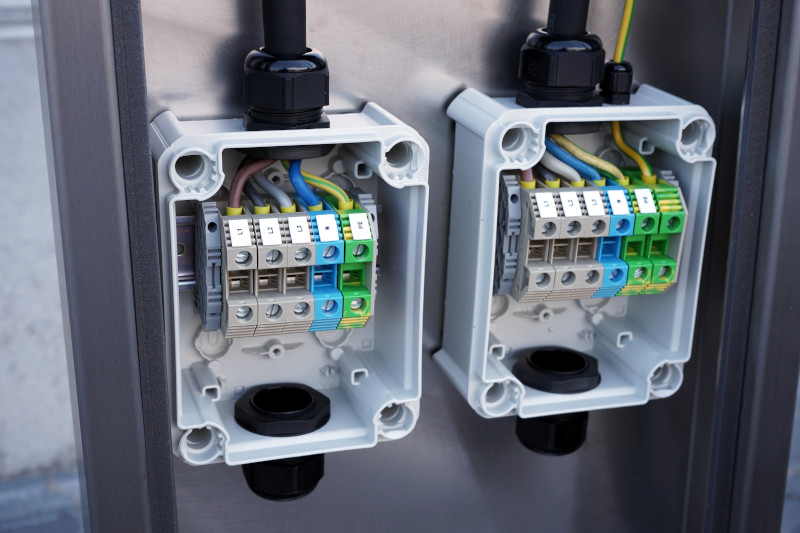
\includegraphics[width=\linewidth]{./img/warp-charger-stand-clamps}
	\end{center}

	Anschließend sind die in der Betriebsanleitung geforderten Prüfungen für die
	Wallboxen durchzuführen.

	\subsubsection{Erdung}
	Die Ladesäule ist unbedingt zu erden. Dazu befindet sich ein Erdungspunkt in
	der Säule auf Höhe der Wallboxen. Dieser ist anzuschließen und die Erdung zu
	überprüfen.

	\subsubsection{RJ45 - Ethernet}
	Zum Anschluss der Ethernetleitung dient ebenfalls ein Verteilergehäuse.
	In dem Gehäuse können die bestehenden Ethernetleitungen der Wallbox
	angeschlossen werden.

	\begin{center}
		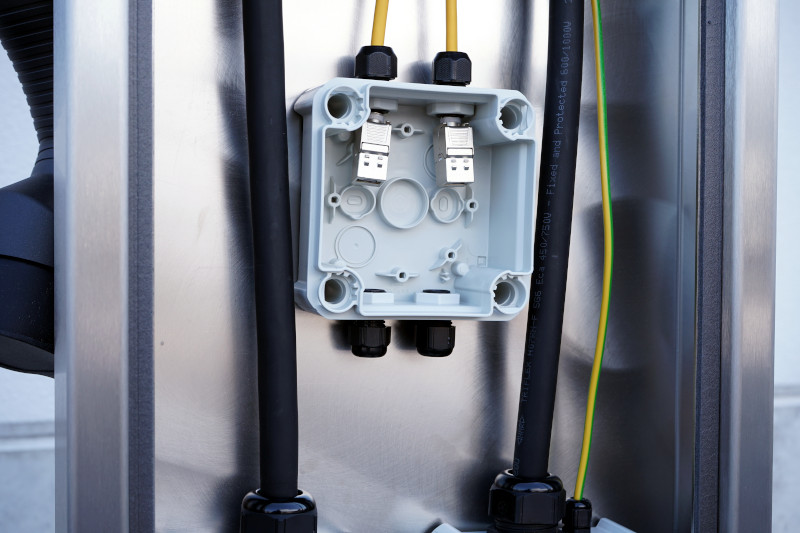
\includegraphics[width=\linewidth]{./img/warp-charger-stand-eth}
	\end{center}

	\section{Inbetriebnahme}
	Die Inbetriebnahme der Ladesäule erfolgt mittels Inbetriebnahme der
	verbauten WARP2 Charger. Weitere Informationen finden sich in der
	Betriebsanleitung der Wallbox.

	\section{Technische Daten}

	%use minipage here to control footnote placement
	\begin{minipage}{\linewidth}

		\begin{description}[leftmargin=!,labelwidth=\widthof{\textbf{Anzahl
		WARP2 Charger}}]
			\setlength{\itemsep}{3pt}
			\item[Material] V4A Edelstahl
			\item[Materialstärke] \SI{1.5}{\milli\meter}
			\item[Anzahl WARP2 Charger] 1-2
			\item[Abmessungen] ca. 344 × 1406 × \SI{102}{\milli\meter} (B/H/T)
			\item[Gewicht] ca. \SI{22}{\kilo\gram} ohne WARP2 Charger
			\item[Zugangsverriegelung]
			      Vierkant, wahlweise mit Schlössern lieferbar
			\item[Lieferumfang] Ladesäule mit gewählten WARP2 Chargern,
			      Bedienungsanleitungen, Montagehilfe inkl. Befestigungsmaterial
		\end{description}
	\end{minipage}

	\section{Kontakt}
	Tinkerforge GmbH\\ Zur Brinke 7\\ 33758 Schloß Holte-Stukenbrock\\
	\begin{description}[leftmargin=!,labelwidth=\widthof{\textbf{Website}}]
		\item[E-Mail] \href{mailto:info@tinkerforge.com}{\texttt{info@tinkerforge.com}}
		\item[Website] \href{https://warp-charger.com}{\texttt{warp-charger.com}}
		\item[Shop] \href{https://tinkerforge.com/de/shop/warp.html}{\texttt{tinkerforge.com/de/shop/warp.html}}
	\end{description}

	\section{Konformitätserklärung}
	Die EU-Konformitätserklärung ist in einem gesonderten Dokument verfügbar.

	\section{Entsorgung}
	\begin{minipage}{0.35\textwidth}
		Die Ladesäule und die Verpackung ist bei Gebrauchsende ordnungsgemäß zu
		entsorgen. Altgeräte dürfen nicht über den Hausmüll entsorgt werden.
	\end{minipage}\hfill
	\begin{minipage}{0.1\textwidth}
		
\includegraphics[width=\linewidth]{./img/weee.pdf}
	\end{minipage}


	\section{Wartung und Reinigung}
	\subsection{Wartung}
	Eine Wartung des Standfußes ist nicht notwendig. 

	\subsection{Reinigung}
	\warn{\textbf{GEFAHR Hohe Spannungen:}\\Gefahr von tödlichen elektrischen
	Stromschlägen. Den Standfuß niemals mit einem Hochdruckreiniger oder einem ähnlichen Gerät reinigen.}
	\begin{itemize}
		\item Anlage nur mit einem feuchten Tuch oder einem Edelstahlreiniger abwischen (Anwendungshinweise des Herstellers beachten). Keine aggressiven Reinigungsmittel, Wachs oder Lösungsmittel verwenden. 
		\item Testen Sie das Reinigungsmittel immer erst an einer unaufälligen Stelle auf Verträgllichkeit.
	\end{itemize}

	\section{Dokumentversionen}
	\begin{tabular}{lll}
		\toprule
		Datum      & Version & Kommentar                   \\
		\midrule
		03.08.2022 & 1.0     & Initialversion              \\
		\bottomrule
	\end{tabular}

	\end{multicols*}

	\section{Anhang}

	\subsection{Herstellung des Fundaments inkl. Zuleitung}
	\label{appendix_base}
	\begin{center}
		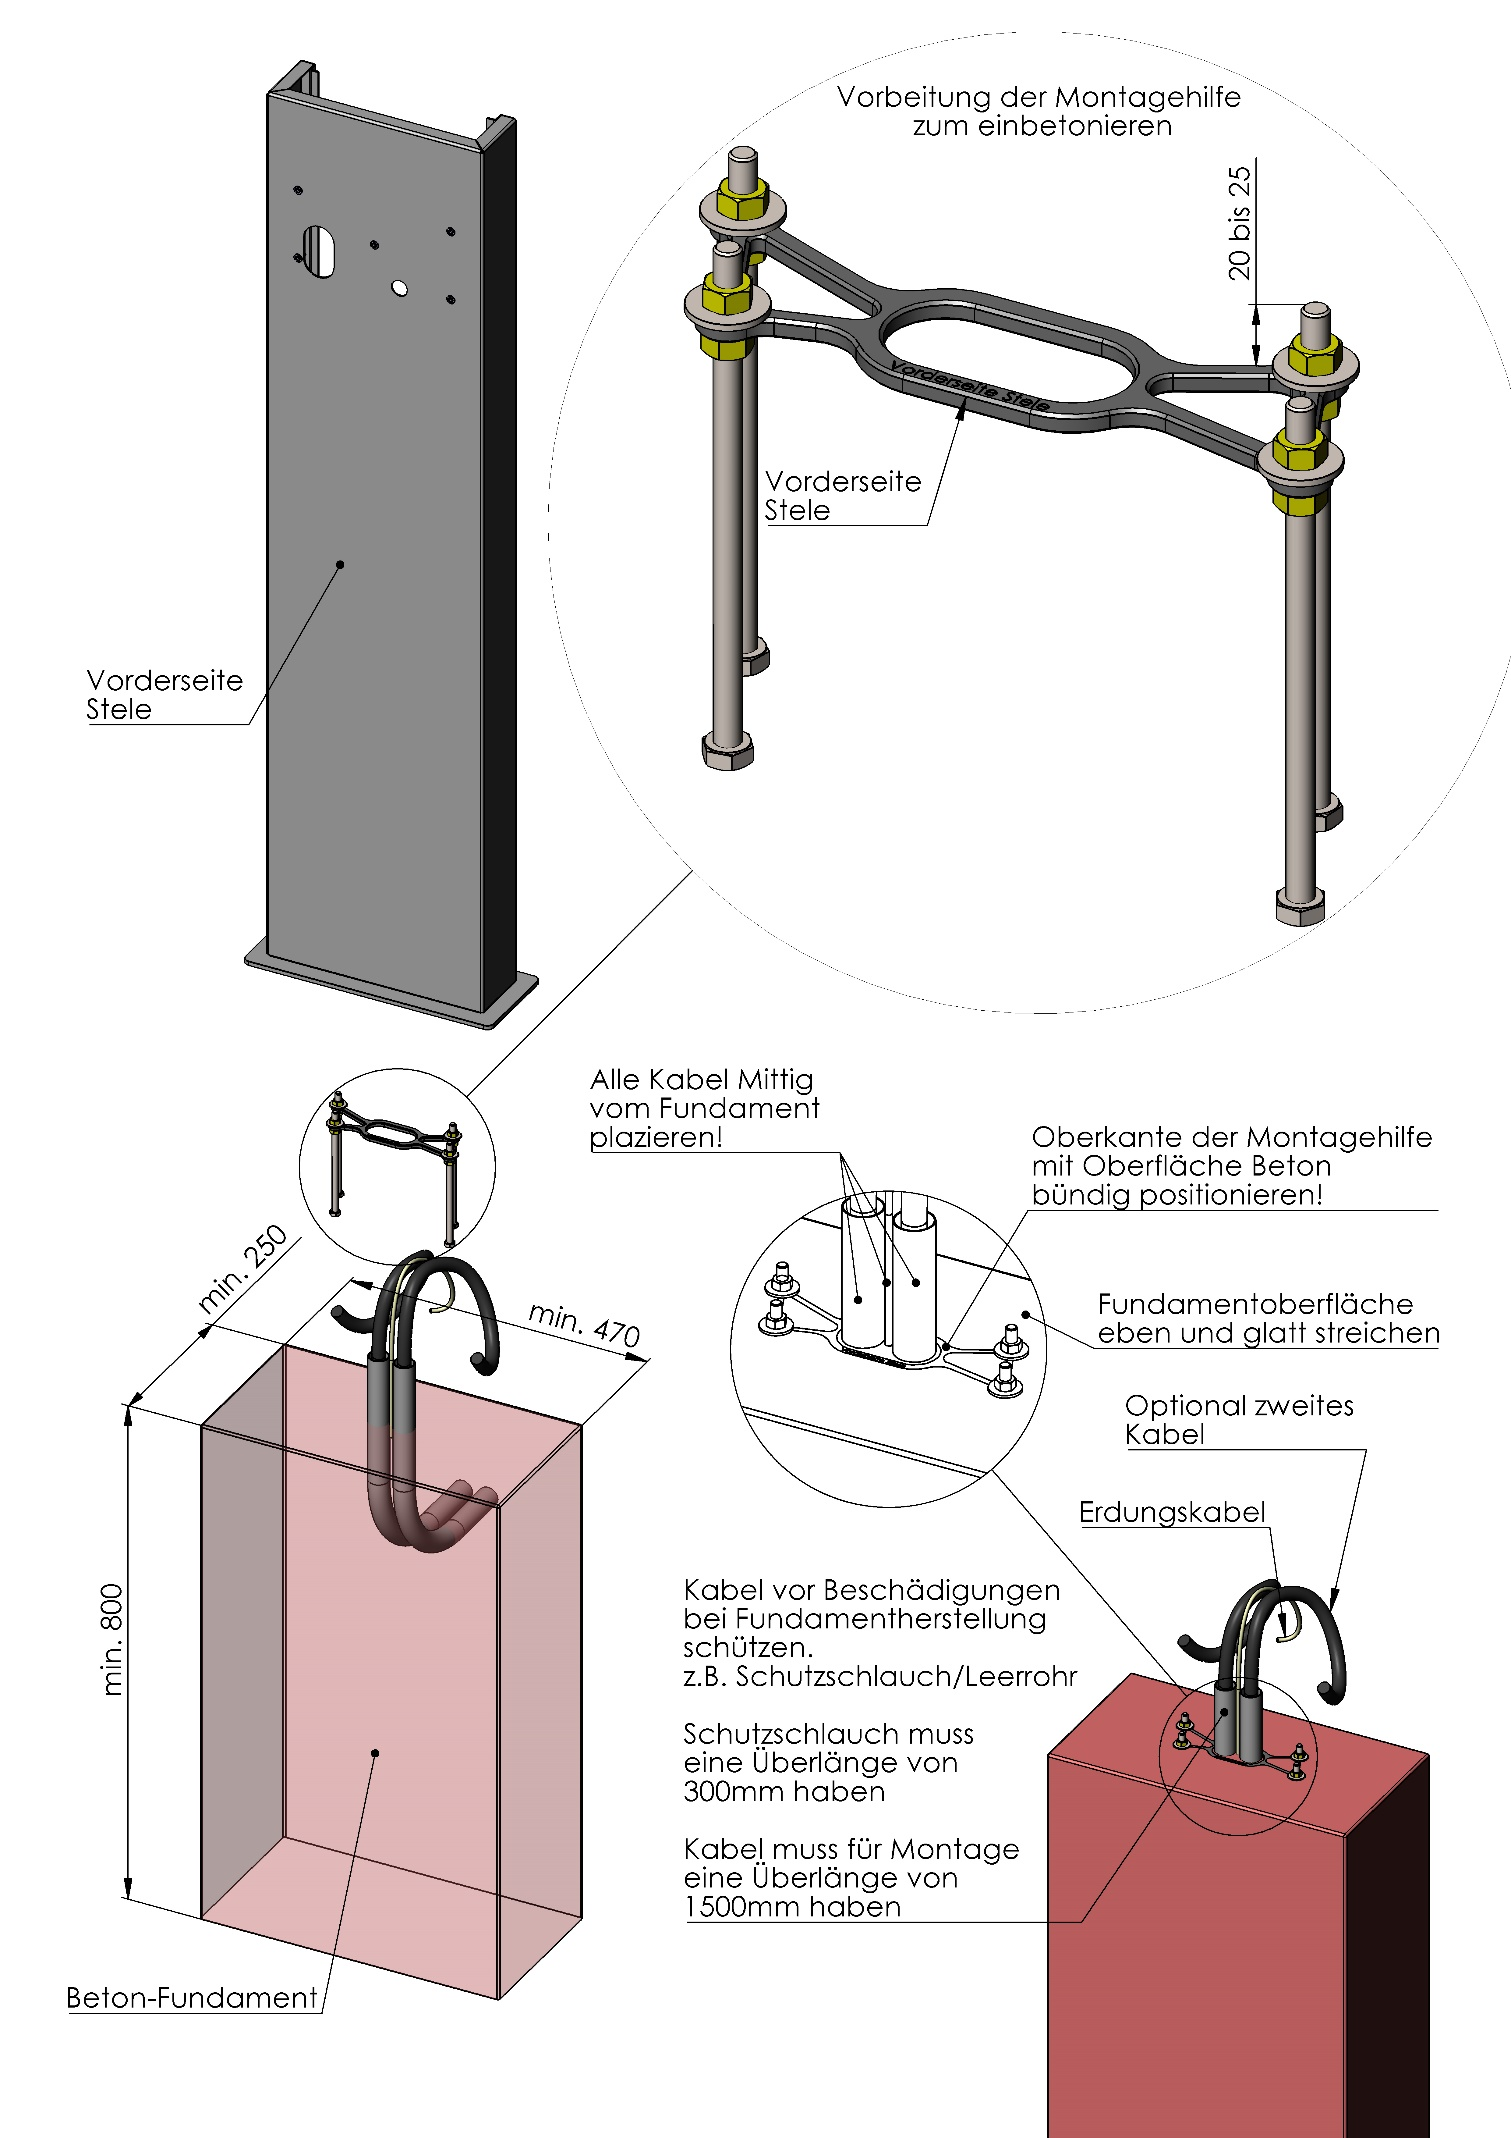
\includegraphics[width=0.9\linewidth]{./img/stand_overview}
	\end{center}

	\subsection{Montage des Standfußes}
	\label{appendix_erection}
	\begin{center}
		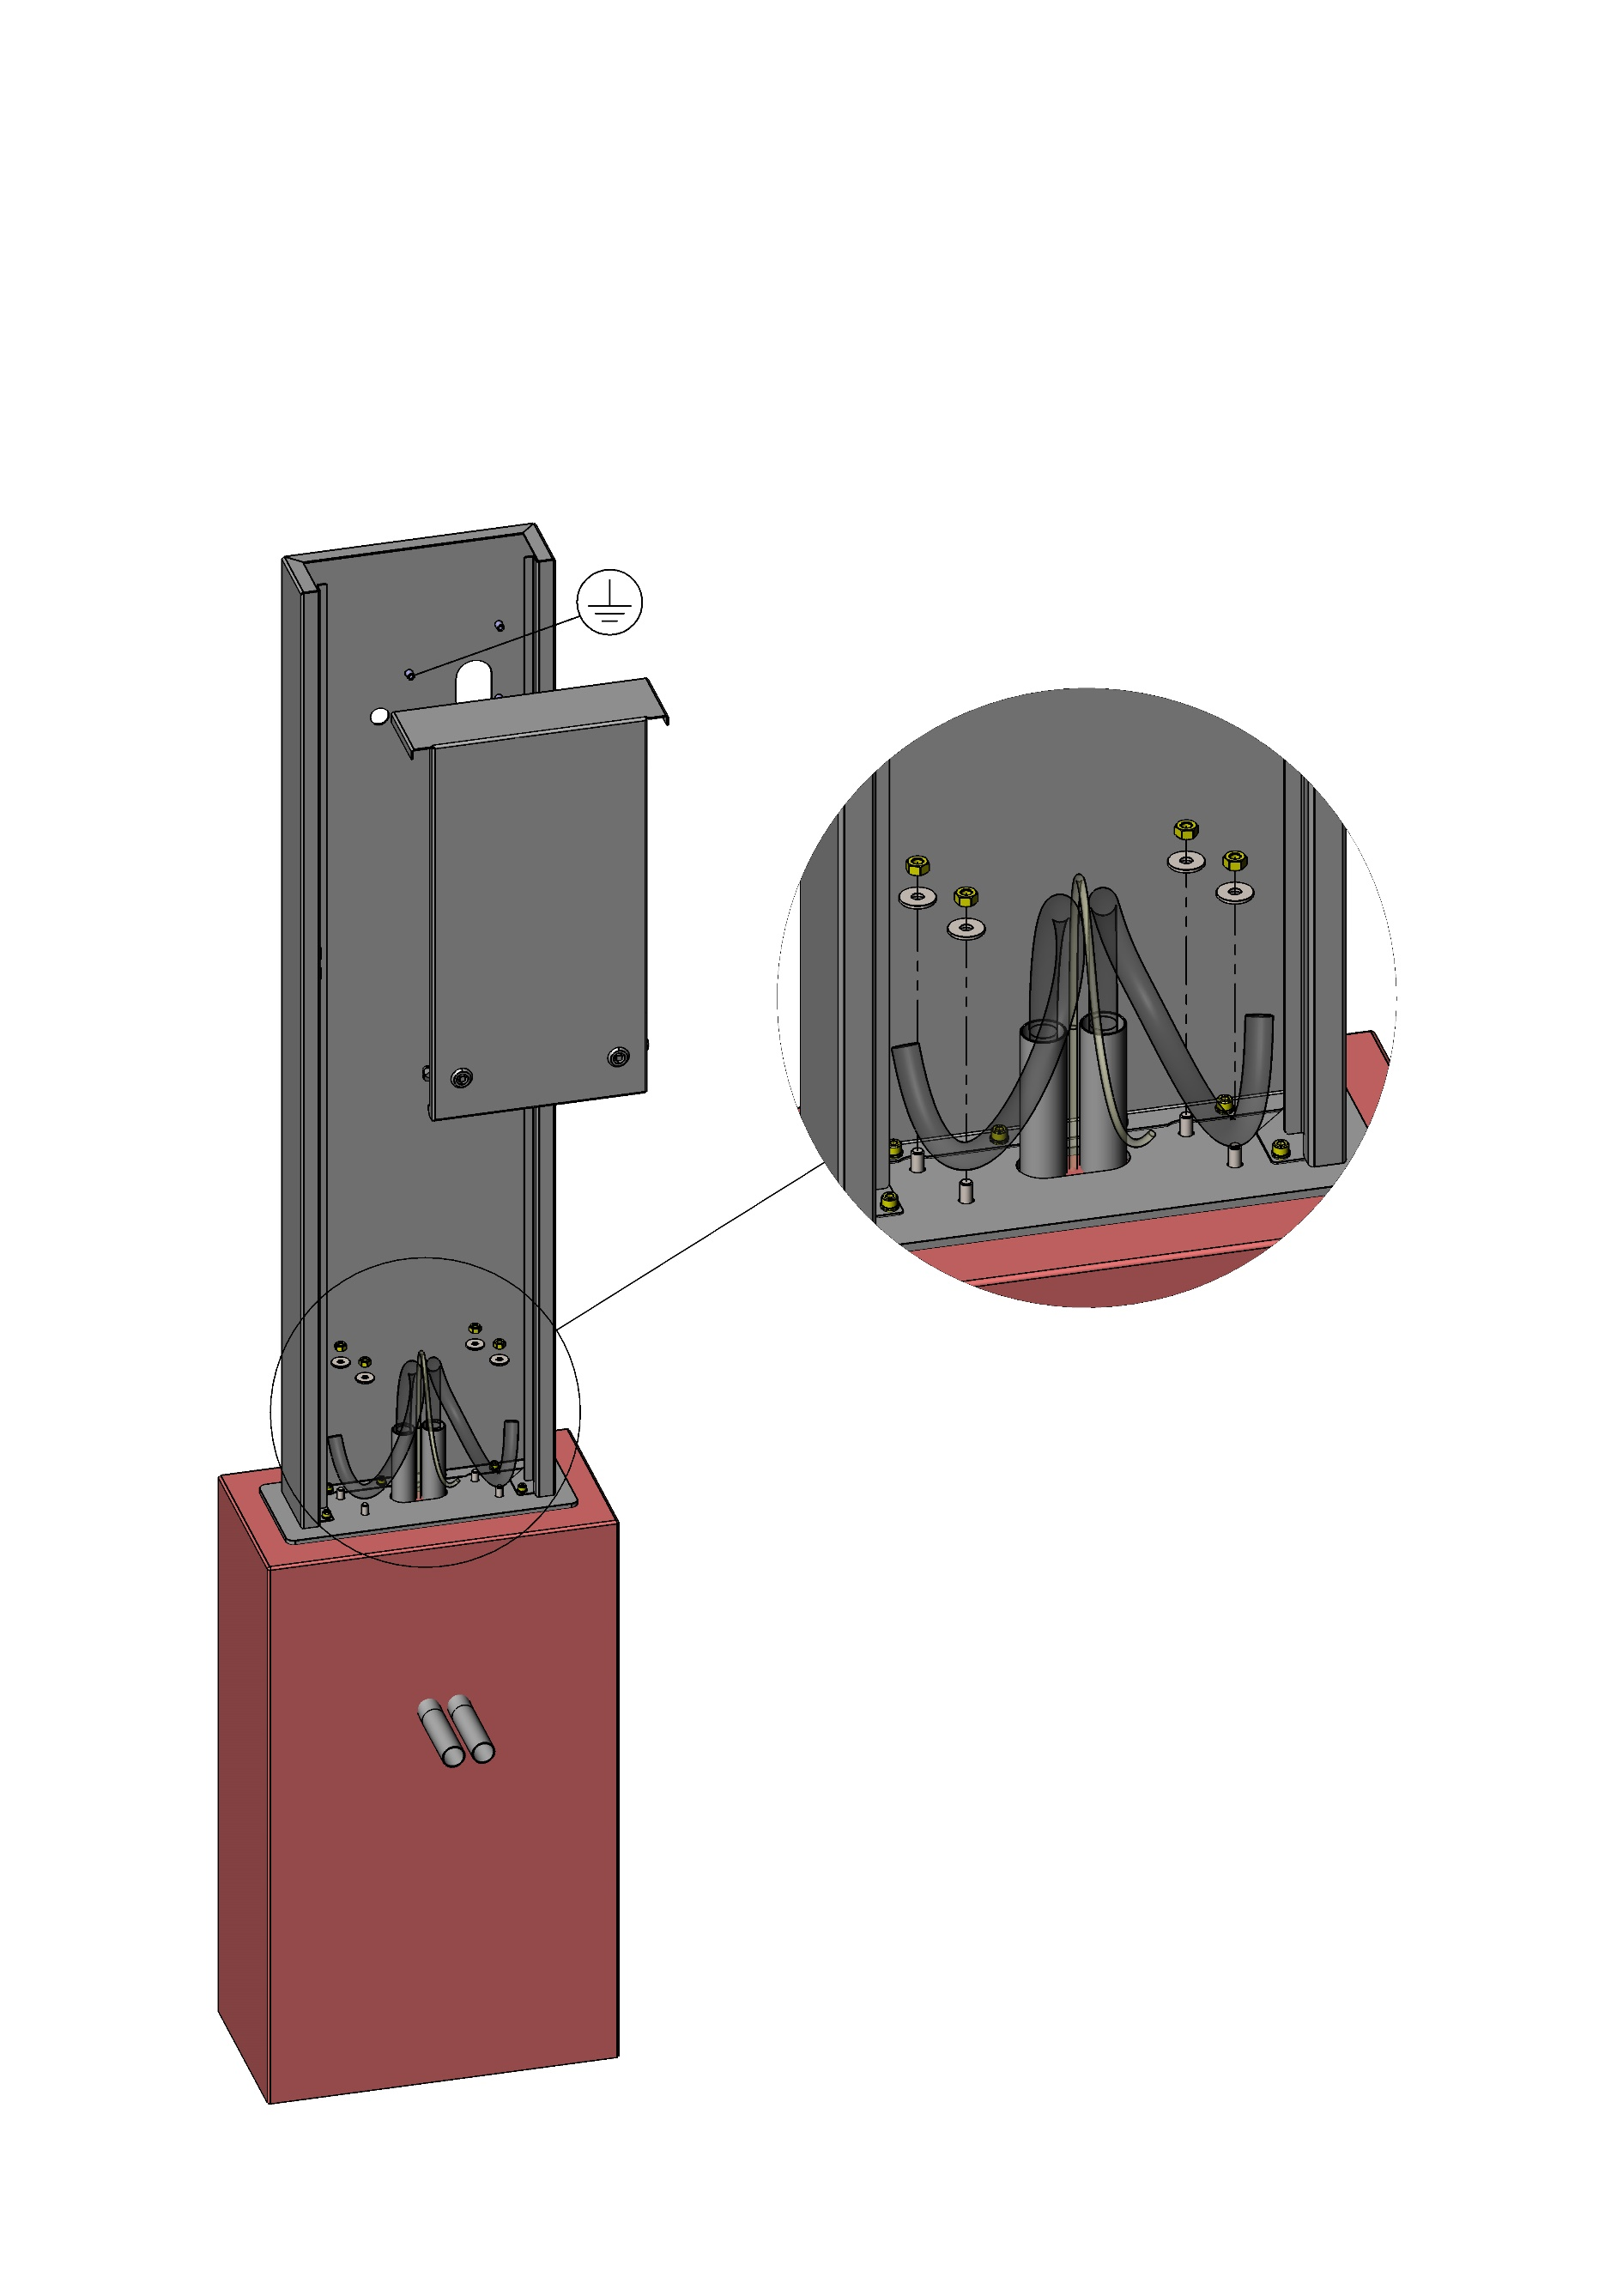
\includegraphics[width=0.9\linewidth]{./img/stand_erection}
	\end{center}

	\subsection{Maße Ladesäule mit einem WARP2 Charger}
	\label{appendix_stand1}
	\begin{center}
		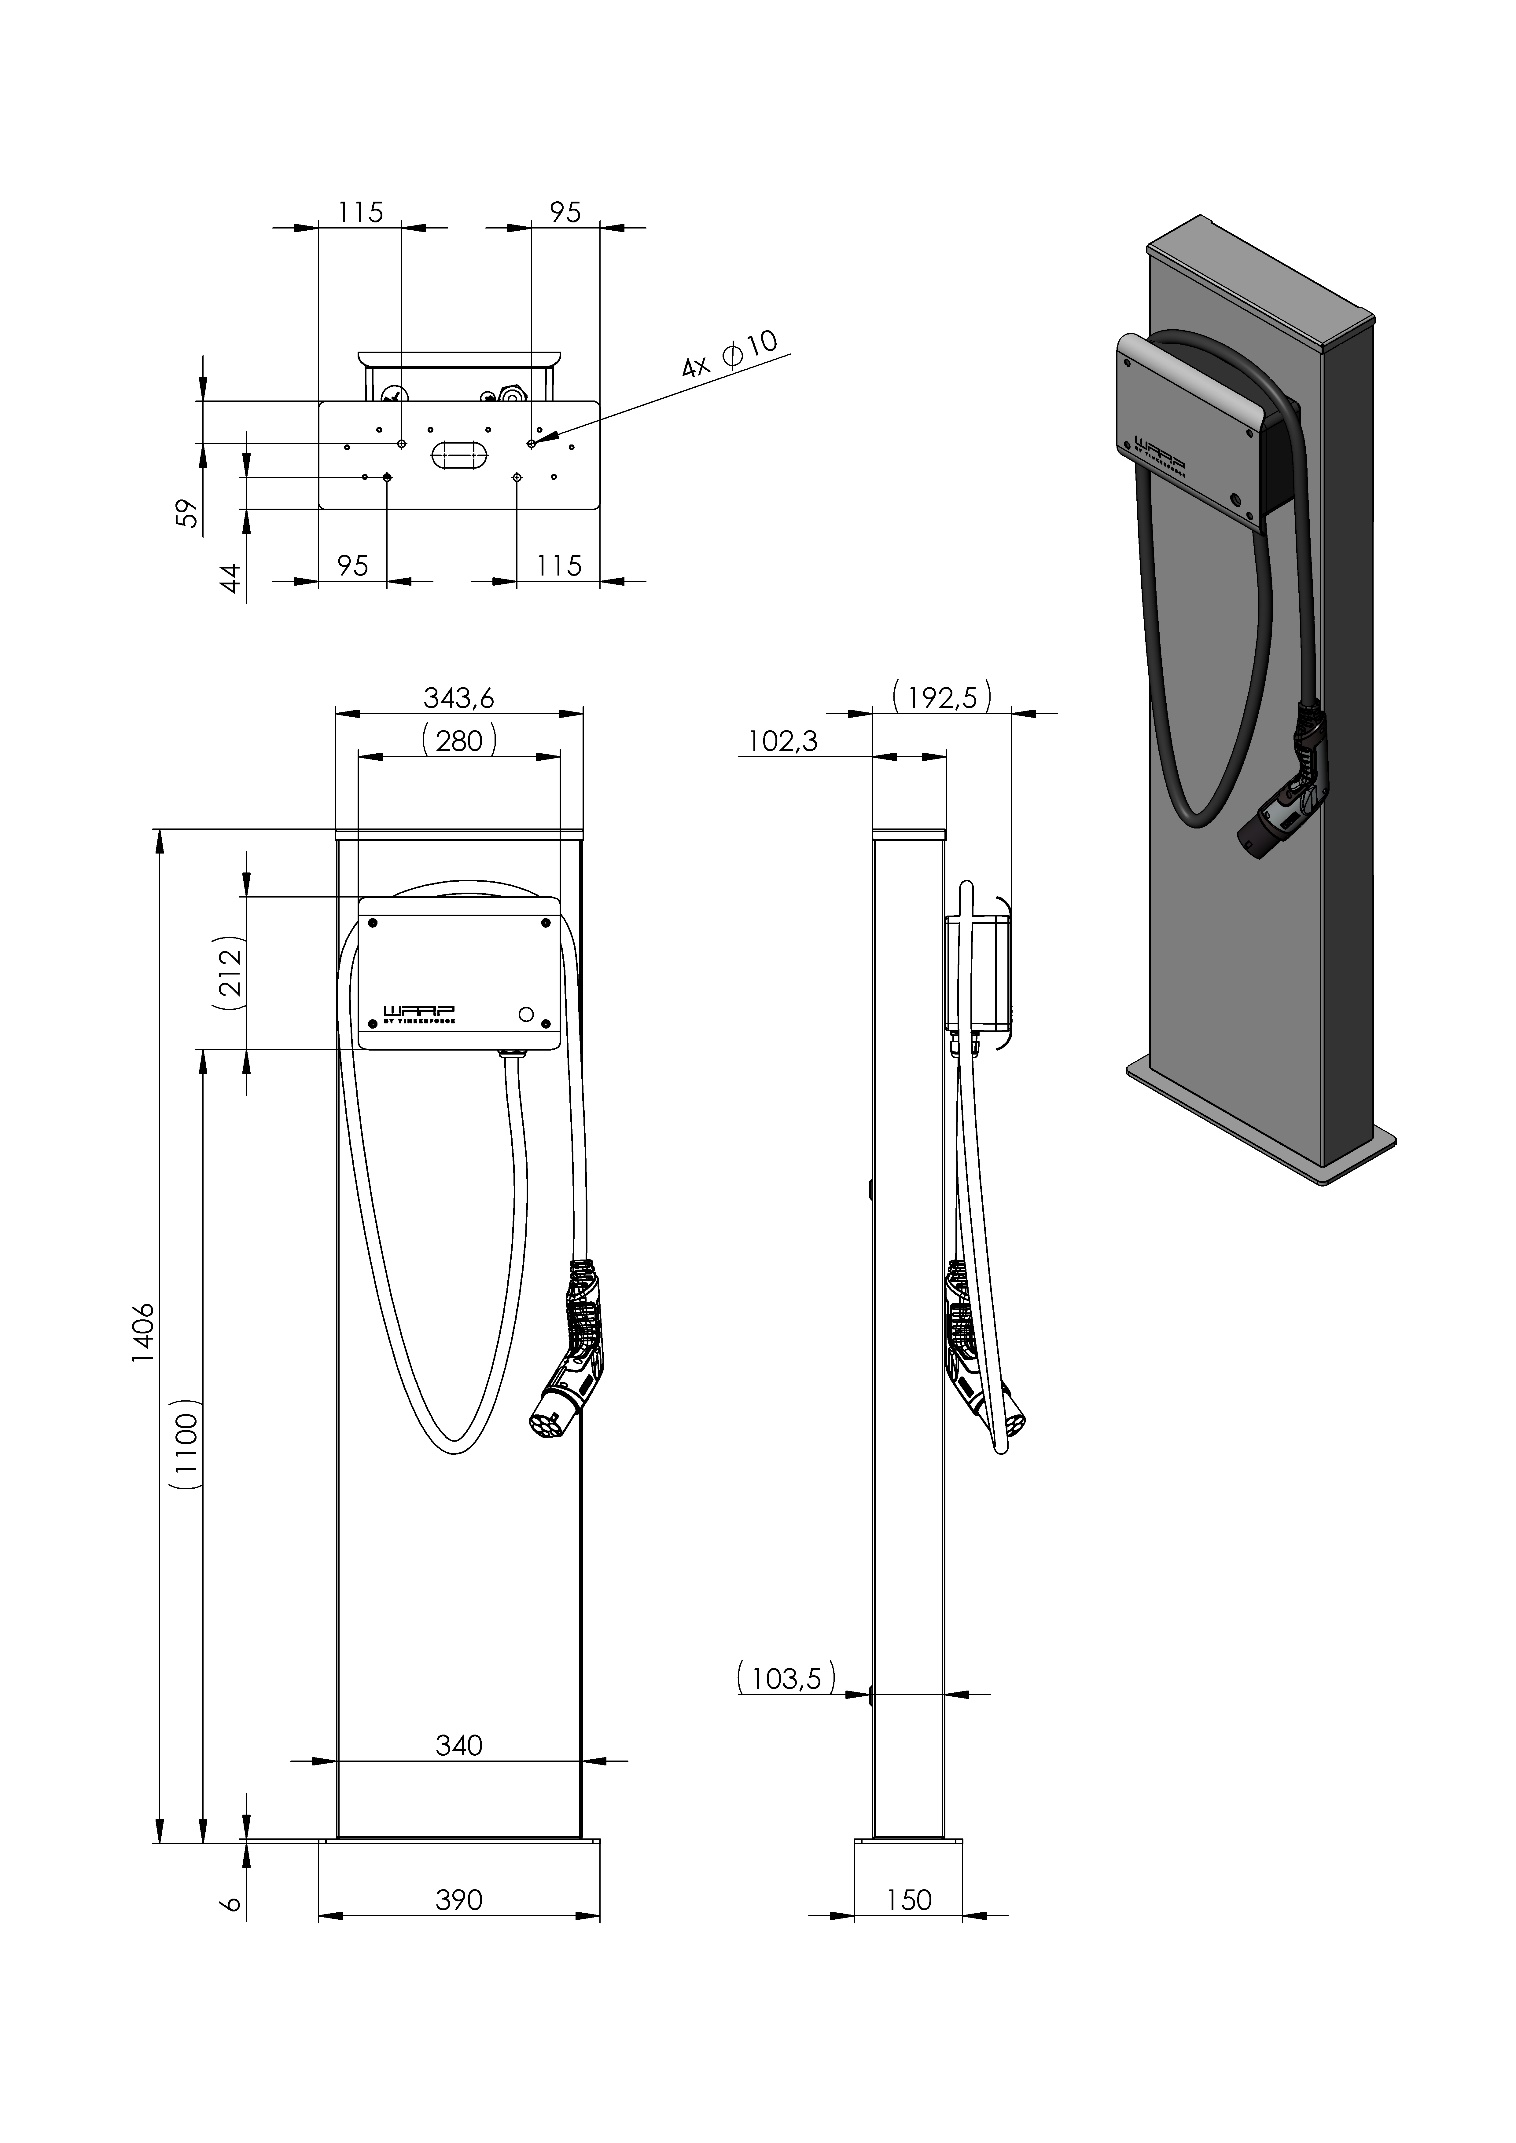
\includegraphics[width=0.9\linewidth]{./img/stand_1}
	\end{center}

	\subsection{Maße Ladesäule mit zwei WARP2 Chargern}
	\label{appendix_stand2}
	\begin{center}
		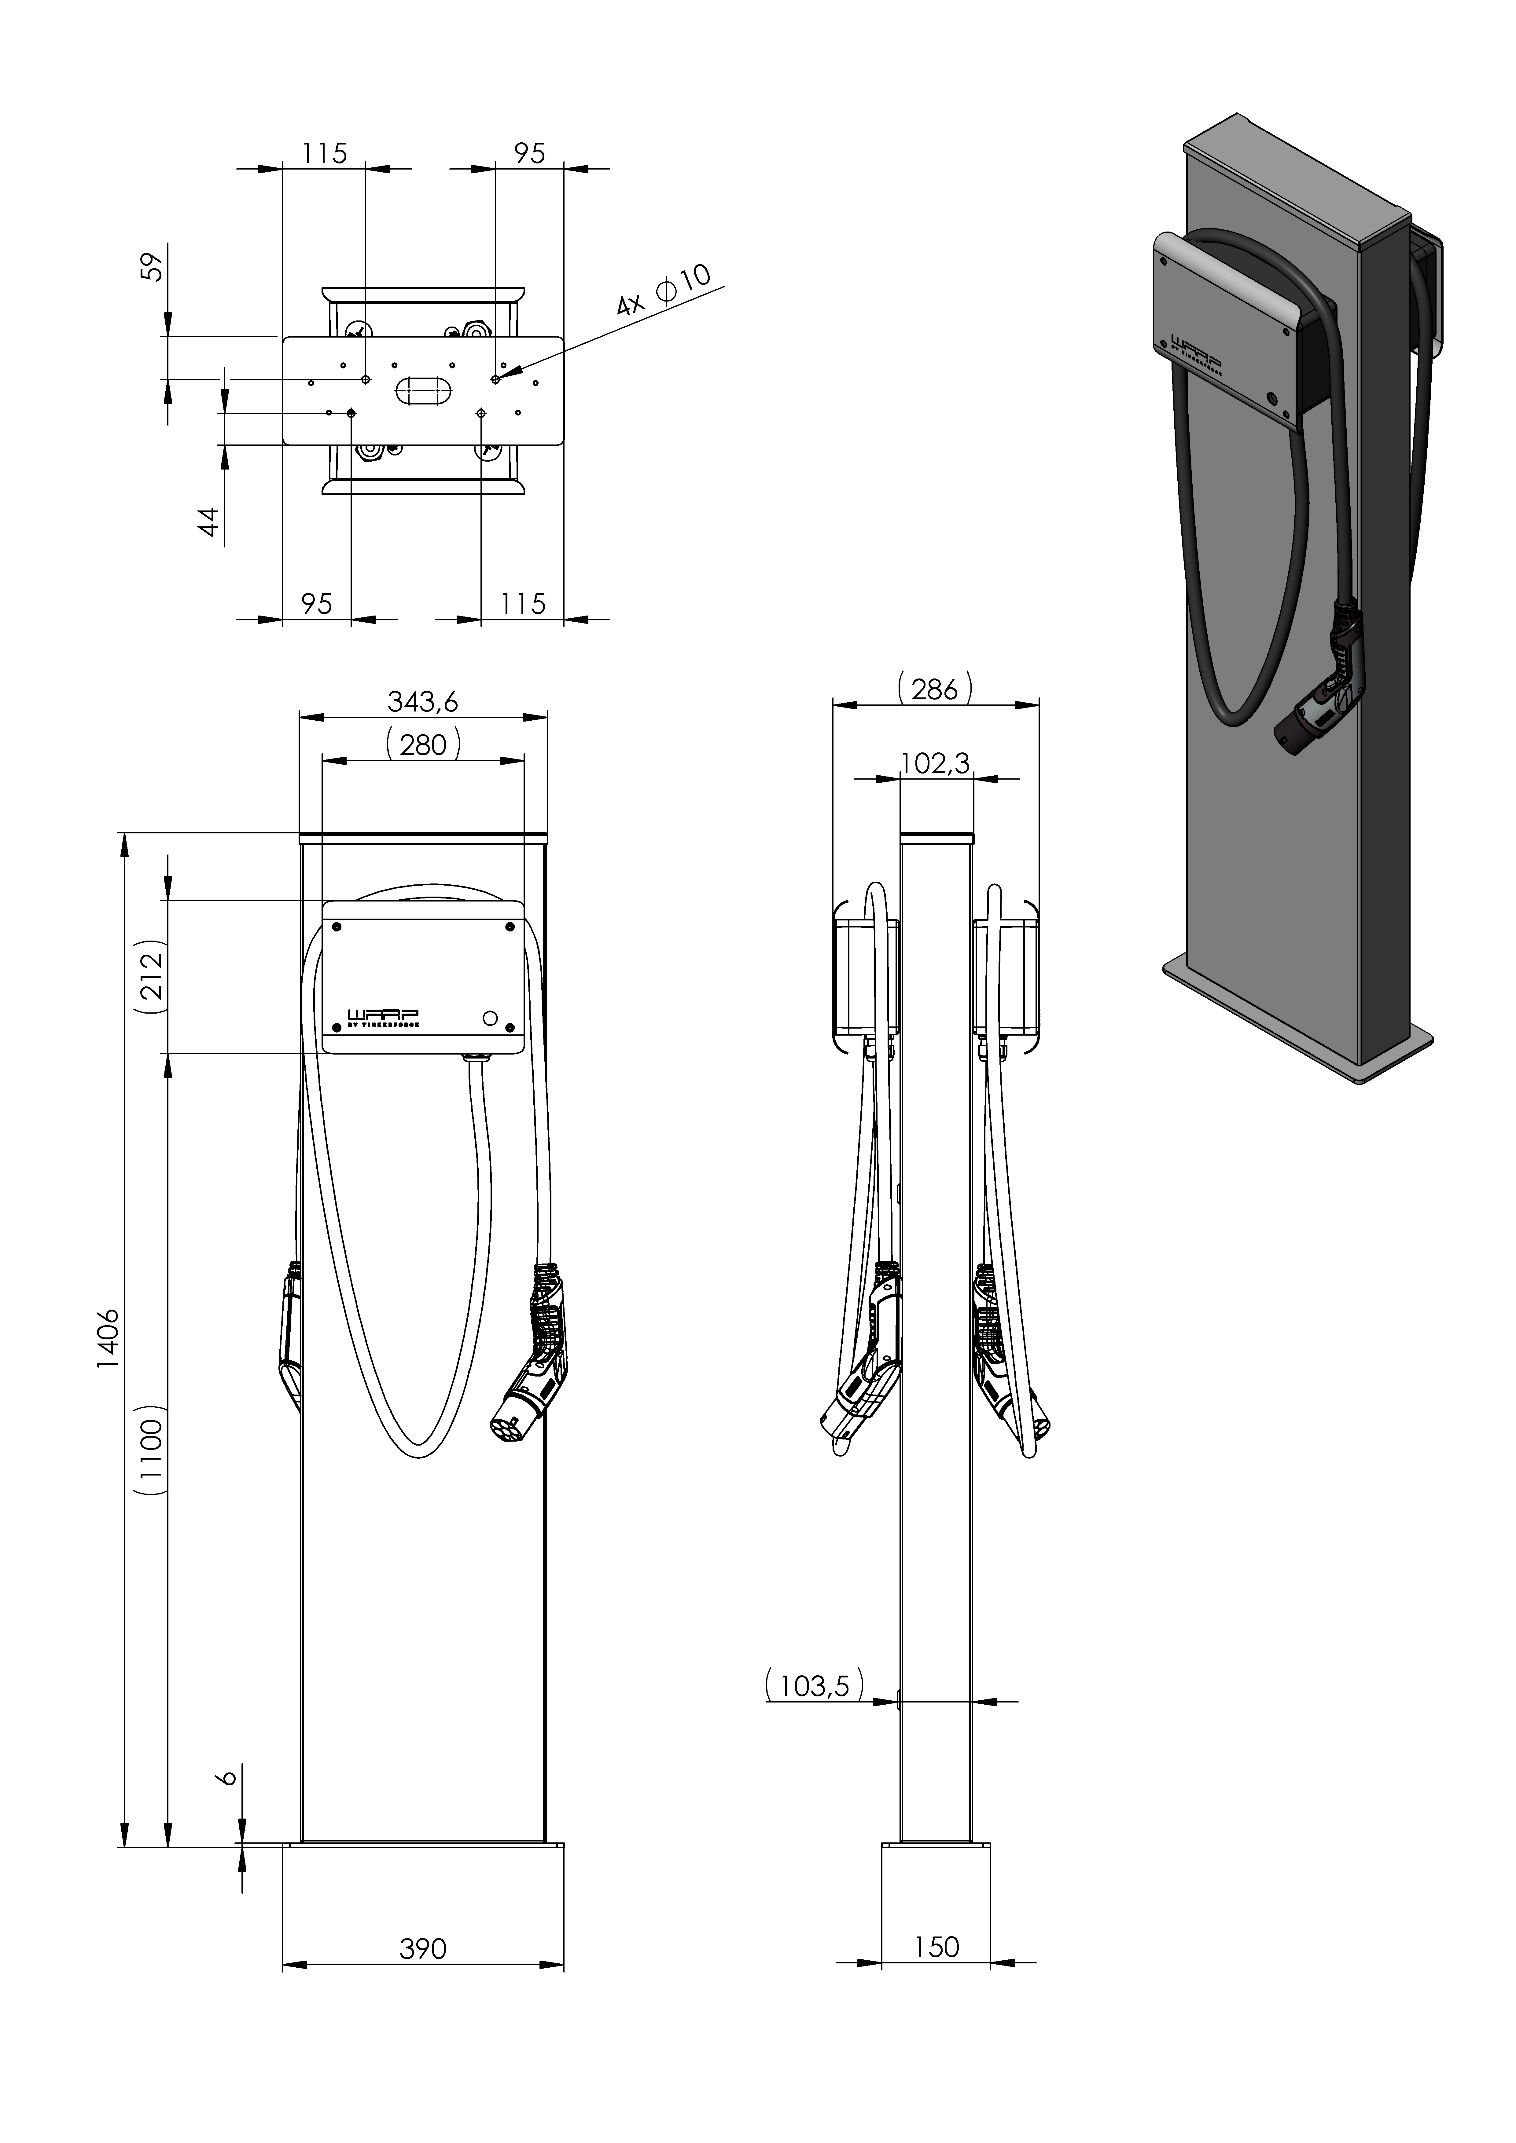
\includegraphics[width=0.9\linewidth]{./img/stand_2}
	\end{center}


\end{document}
